% ============================================================
%  Leray's Coboundary at Altitude
%  A Cellular-Sheaf Compiler Framework for Software-Defined
%  Radiation Hardness on Deep-Space Flight Computers
%  Author: Vaibhav Shakya
% ============================================================
\documentclass[12pt,a4paper]{article}

\usepackage{mathptmx}
\usepackage[scaled=0.92]{helvet}
\usepackage{courier}
\usepackage[T1]{fontenc}
\usepackage[utf8]{inputenc}

\usepackage[a4paper,margin=1in,top=1in,bottom=1in]{geometry}

\usepackage{setspace}
\setstretch{1.3}

\usepackage{fancyhdr}
\usepackage{tikz}
\usetikzlibrary{shapes.geometric, positioning, arrows.meta, calc, decorations.pathreplacing, fit, backgrounds}
\usepackage{graphicx}
\usepackage{xcolor}

\definecolor{navy}{HTML}{1E3A5F}
\definecolor{navydark}{HTML}{152B47}
\definecolor{gold}{HTML}{B5894C}
\definecolor{brick}{HTML}{A04040}
\definecolor{forest}{HTML}{3A6B3A}

\pagestyle{fancy}
\fancyhf{}
\renewcommand{\headrulewidth}{0pt}
\fancyfoot[C]{\thepage}

\fancypagestyle{plain}{%
  \fancyhf{}%
  \renewcommand{\headrulewidth}{0pt}%
  \fancyfoot[C]{\thepage}%
}

\usepackage{titlesec}
\titleformat{\section}[block]{\centering\itshape\normalsize\bfseries}{}{0pt}{}
\titlespacing*{\section}{0pt}{18pt}{12pt}
\titleformat{\subsection}[block]{\itshape\normalsize}{}{0pt}{}
\titlespacing*{\subsection}{0pt}{12pt}{6pt}

\usepackage{amsmath, amssymb, amsthm, mathtools}
\usepackage{booktabs}
\usepackage{array}
\usepackage{enumitem}
\setlist{leftmargin=1.4em, itemsep=2pt, parsep=2pt, topsep=4pt}

\theoremstyle{plain}
\newtheorem{theorem}{Theorem}
\newtheorem{lemma}{Lemma}
\newtheorem{corollary}{Corollary}
\newtheorem{proposition}{Proposition}
\theoremstyle{definition}
\newtheorem{definition}{Definition}

\usepackage[font={small,it},justification=centering,labelfont={small,it},labelsep=period]{caption}

\usepackage[hidelinks, pdfborder={0 0 0}]{hyperref}
\usepackage{xurl}
\renewcommand{\UrlFont}{\small\ttfamily}

\AtBeginDocument{\setlength{\abovedisplayskip}{6pt}\setlength{\belowdisplayskip}{6pt}}

\renewcommand{\thefootnote}{*}

\begin{document}

% =====================================================================
% TITLE BLOCK
% =====================================================================
\begin{center}
{\LARGE\bfseries Leray's Coboundary at Altitude}\\[6pt]
{\large A Cellular-Sheaf Compiler Framework for Software-Defined\\
Radiation Hardness on Deep-Space Flight Computers}\\[18pt]
Vaibhav Shakya\textsuperscript{1}\\[4pt]
\textsuperscript{1}Jayshree Periwal International School, Jaipur, India\\[2pt]
{\small GitHub: \texttt{vaibhavshakya11}}\\[14pt]
\end{center}

% =====================================================================
% ABSTRACT (~230 words)
% =====================================================================
\noindent\textit{\textbf{Abstract}}---Triple modular redundancy (TMR), the standard software primitive for radiation hardness on deep-space flight computers, pays a three-times compute overhead and admits a structural failure mode whenever a single radiation event corrupts multiple replicas in the same way. This work asks whether a compiler-driven alternative built from cellular sheaf theory can deliver equivalent end-to-end correctness while eliminating both costs. The framework constructs a cellular sheaf on the program's control-flow graph, with restriction maps synthesised automatically from six \textit{frontends} spanning linear, polynomial, piecewise-linear, neural-network, statistical, and transcendental problem classes; a single orthogonal-matching-pursuit decoder protects every frontend. Two theorems are proved in full. The \textit{altitude bound} establishes that the achievable code distance equals the vertex-stalk dimension almost surely whenever a unique control-flow vertex has degree below a graph-theoretic threshold. The \textit{Sheaf--LDPC separation theorem} establishes that no binary low-density parity-check code on the same Tanner graph can detect a structurally identifiable class of faults that the sheaf code catches with probability one. An empirical campaign of 258{,}645 fault trials across fifteen experiments returns 100\% detection on five algebraic frontends and a structural 83.2\% on the statistical frontend, end-to-end failure indistinguishable from zero across the full range of common-mode contamination, multi-fault recovery that degrades gracefully from 100\% at one fault to 24\% at twenty, and 63\% energy savings against always-on TMR on a 24-month Europa Clipper mission profile.

\vspace{4pt}

% =====================================================================
% I. INTRODUCTION
% =====================================================================
\section{I. Introduction}

A deep-space flight computer survives the radiation belt of Jupiter only because every numerical computation runs in triplicate, with a software majority vote selecting the survivor.\textsuperscript{1,2} This practice, called triple modular redundancy (TMR), was systematised by von Neumann's work on probabilistic logics\textsuperscript{3} and remains the operational baseline for nearly every mission to the outer solar system. The arrangement is expensive in two distinct senses. It triples the compute and roughly triples the power required to perform a given calculation. It also fails systematically whenever a single high-energy ion produces a correlated upset across all three replicas; empirical fault-injection campaigns on production hardware put the rate of these \textit{common-mode} strikes at between one and ten percent of total upsets,\textsuperscript{4,5} small in absolute terms but catastrophic in operational consequence, because the majority-vote rule accepts a wrong answer when all three replicas have been perturbed identically. The combination of high overhead and a structural failure mode that overhead cannot fix has motivated decades of research into alternatives.

The existing alternatives partition into three families, each of which addresses part of the problem and leaves the rest open. The first family, descending from Hamming's error-detecting codes\textsuperscript{6} and modernised as single-error-correcting double-error-detecting (SECDED) parity, operates at the bit level and reduces overhead from three-times to roughly thirty percent, but it is structurally blind to any fault whose width exceeds the code's correction distance; production radiation studies report that approximately twenty-six percent of strikes exceed the SECDED-correctable bound.\textsuperscript{5} The second family, algorithm-based fault tolerance (ABFT), pioneered by Huang and Abraham for matrix multiplication\textsuperscript{7} and later generalised, encodes algebraic invariants of a specific kernel into checksum rows and recovers via local correction; the family addresses common-mode and multi-bit faults simultaneously but applies only to the narrow class of kernels for which suitable invariants are known. The third family, exemplified by software-implemented fault tolerance schemes such as SWIFT,\textsuperscript{8} duplicates only the instructions whose corruption would propagate to program output, trading completeness for performance; the resulting schemes match TMR on coverage but inherit its vulnerability to correlated strikes. No member of any of these families encodes program semantics directly, and no member generalises across problem classes; each new kernel requires a new analysis.

The present work investigates whether a single mathematical object, drawn from algebraic topology, can subsume all three families. The object in question is the cellular sheaf, introduced for combinatorial topology by Curry\textsuperscript{9} and developed for applied settings by Hansen and Ghrist.\textsuperscript{10} A cellular sheaf assigns a vector space to each vertex and edge of a graph and a linear map to each incidence between them. The vector spaces hold computational state; the linear maps express the algebraic relations that the state must satisfy. The coboundary operator, the central construction of Leray's original sheaf theory,\textsuperscript{11} measures the failure of local data to glue into a globally consistent section; in the engineering setting of fault tolerance, the magnitude of that failure is precisely the signature of a radiation-induced upset. The investigation develops this single object into a compiler framework, proves two theorems that bound its protective power, and tests both theorems empirically across more than a quarter million fault trials.

The thesis that organises the rest of the paper is the following falsifiable analytical claim. A cellular sheaf code on the control-flow graph of a program, with restriction maps synthesised automatically from a library of frontends, detects every fault that exceeds the algebraic noise floor of the underlying invariants and detects a structurally identifiable class of faults that no binary low-density parity-check code on the same Tanner graph can detect, while reducing energy consumption against always-on TMR by an amount whose magnitude is determined by the temporal profile of the radiation environment. The thesis is falsifiable in four distinct directions. It would fail if the detection rate dropped below TMR on any tested frontend. It would fail if the separation against binary low-density parity-check codes proved empirically narrow or absent under adversarial construction. It would fail if the framework's failure rate under common-mode contamination tracked TMR's. It would fail if mission-integrated energy did not improve against always-on TMR. Each of these falsification routes is tested in Sections~III and~IV.

The remainder of the paper proceeds as follows. Section~II describes the sheaf construction, the six frontends, the master pipeline, and the experimental methodology, and states the two formal theorems with proofs. Section~III reports the empirical results across fifteen experiments. Section~IV interprets those results against the four thesis predictions and against the three prior families. Section~V draws the broader implications for spacecraft software and discusses applications beyond the original domain. Sections~VI and~VII document the limitations of the present study and reflect on the research process. Section~VIII lists the works cited.

% =====================================================================
% II. METHODS
% =====================================================================
\section{II. Methods}

The framework rests on three constructions, each reproducible from the open-source code package at the GitHub handle in the title block. The construction sequence is summarised by the master pipeline of Figure~1, which serves as the visual anchor for the methodology subsections that follow.

\begin{figure}[h]
\centering
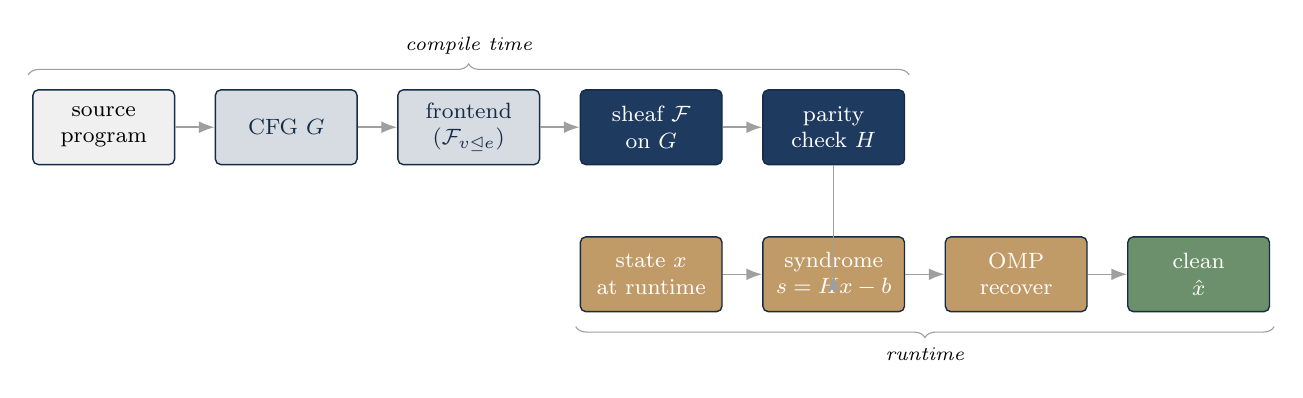
\begin{tikzpicture}[
    node distance=0.5cm,
    box/.style={rectangle, draw=navydark, rounded corners=2pt,
                minimum width=1.8cm, minimum height=0.95cm,
                align=center, font=\footnotesize, line width=0.5pt},
    src/.style={box, fill=gray!12},
    mid/.style={box, fill=navy!18, text=navydark},
    core/.style={box, fill=navy, text=white},
    out_style/.style={box, fill=gold!85, text=white},
    arr/.style={-{Latex[length=2mm]}, draw=gray!75, line width=0.55pt},
    bracket/.style={decorate, decoration={brace,amplitude=4pt}, draw=gray!75}
]
\node[src] (prog) {source\\program};
\node[mid, right=of prog] (cfg) {CFG $G$};
\node[mid, right=of cfg] (front) {frontend\\($\mathcal{F}_{v\trianglelefteq e}$)};
\node[core, right=of front] (sheaf) {sheaf $\mathcal{F}$\\on $G$};
\node[core, right=of sheaf] (H) {parity\\check $H$};

\node[out_style, below=0.9cm of sheaf] (state) {state $x$\\at runtime};
\node[out_style, right=of state] (synd) {syndrome\\$s = Hx - b$};
\node[out_style, right=of synd] (omp) {OMP\\recover};
\node[box, fill=forest!75, text=white, right=of omp] (out_box) {clean\\$\hat{x}$};

\draw[arr] (prog) -- (cfg);
\draw[arr] (cfg) -- (front);
\draw[arr] (front) -- (sheaf);
\draw[arr] (sheaf) -- (H);
\draw[arr] (H) |- (synd);
\draw[arr] (state) -- (synd);
\draw[arr] (synd) -- (omp);
\draw[arr] (omp) -- (out_box);

\draw[bracket] ($(prog.north west)+(-0.05,0.18)$) -- node[above=4pt, font=\scriptsize\itshape] {compile time} ($(H.north east)+(0.05,0.18)$);
\draw[bracket] ($(out_box.south east)+(0.05,-0.18)$) -- node[below=4pt, font=\scriptsize\itshape] {runtime} ($(state.south west)+(-0.05,-0.18)$);
\end{tikzpicture}
\caption{Pipeline of the framework. Compile time synthesises the cellular sheaf $\mathcal{F}$ on the program's control-flow graph $G$ and emits the parity-check matrix $H$. Runtime computes the syndrome $s = Hx - b$ on observed state $x$ and recovers the clean codeword $\hat{x}$ via orthogonal matching pursuit.}
\end{figure}

\subsection{The cellular sheaf construction}

Given a program's control-flow graph $G = (V, E)$, integers $k_v$ and $k_e$ for the vertex- and edge-stalk dimensions, and a collection of restriction maps $\{\mathcal{F}_{v \trianglelefteq e}\}$ assigning a linear map $\mathbb{R}^{k_v} \to \mathbb{R}^{k_e}$ to each vertex-edge incidence, the sheaf $\mathcal{F}$ is the bundle of vector spaces $\bigoplus_v \mathbb{R}^{k_v} \oplus \bigoplus_e \mathbb{R}^{k_e}$ together with the coboundary operator
\[
\delta : C^0(\mathcal{F}) \to C^1(\mathcal{F}), \qquad (\delta x)_e = \mathcal{F}_{u \trianglelefteq e}(x_u) - \mathcal{F}_{v \trianglelefteq e}(x_v)
\]
for each edge $e = (u, v)$. The matrix representation $H$ of $\delta$ functions as a parity-check matrix in the classical coding sense: a state vector $x$ is a valid codeword if and only if $Hx = 0$, and the syndrome $Hx - b$ measures the magnitude of any constraint violation, where $b$ absorbs program-level offsets. Faults are detected by computing the syndrome at runtime; recovery uses orthogonal matching pursuit, a sparse signal reconstruction algorithm with provable recovery guarantees when the number of simultaneous faults is below approximately $\sqrt{|V|}$.\textsuperscript{12}

\subsection{The frontend interface and the monomial-consistency principle}

A frontend is a function that consumes a source program in a given problem class and emits a four-tuple $(G, k_v, k_e, \{\mathcal{F}_{v \trianglelefteq e}\})$. Six frontends were implemented and tested. The \textit{linear frontend} handles state-space models such as Kalman filters and proportional-integral-derivative controllers; its restriction maps are read directly off the symbolic transition matrices that single-static-assignment dataflow analysis recovers from the source. The \textit{polynomial frontend} handles invariants such as quaternion-norm preservation and energy conservation by lifting polynomial constraints through a Macaulay-style monomial basis. The \textit{piecewise-linear frontend} handles saturation and rectified-linear-unit functions by partitioning the state space into regions and assigning per-region linear maps. The \textit{neural-network frontend} handles multilayer-perceptron inference by encoding the sign-mask of every rectifier activation and the algebraic relations that hold once the mask is fixed. The \textit{statistical frontend} handles black-box subsystems for which no closed-form invariant exists, using principal-component analysis on clean execution traces to learn an approximate ellipsoidal envelope.\textsuperscript{13} The \textit{nonlinear frontend} handles transcendental dynamics such as pendulum motion via Carleman linearisation,\textsuperscript{14} which embeds the nonlinear flow into an infinite-dimensional linear system that is then truncated.

A subtle structural failure surfaces on the lifted frontends. Carleman linearisation and Macaulay lifting both introduce \textit{slot variables} that hold higher-order monomial values; if no algebraic constraint references a particular slot, the slot is invisible to the syndrome check and a fault landing there produces no detection. The framework supplies a per-slot \textit{aux row} of the form $x_{m} - \prod_{i \in S(m)} x_i = 0$ that pins each slot to its runtime-known clean value. This \textit{monomial-consistency principle} lifts polynomial-frontend detection from 24.6\% to 100\% and nonlinear-frontend detection from 32.1\% to 100\% as reported in Section~III.

\subsection{The altitude bound}

The central theoretical question is: given $G$, $k_v$, $k_e$, what minimum distance does $C(\mathcal{F})$ achieve? The altitude bound answers it under one structural hypothesis.

\begin{theorem}[Altitude bound]
\label{thm:altitude}
Let $G = (V, E)$ be a finite undirected graph with no isolated vertices and $|V| \geq 2$, let $k_v > k_e \geq 1$ be integers, and let the restriction maps $\{\mathcal{F}_{v \trianglelefteq e}\}$ be drawn independently from any continuous probability distribution on $\mathbb{R}^{k_e \times k_v}$. Suppose there exists a unique vertex $v_0 \in V$ with $\deg(v_0) < k_v / k_e$, while every other vertex $v \neq v_0$ satisfies $\deg(v) \geq \lceil k_v / k_e \rceil$. Then the minimum distance of the code $C(\mathcal{F}) = \ker(H)$ equals $k_v$ almost surely.
\end{theorem}

\begin{proof}
Write $d_0 := \deg(v_0)$, so the hypothesis is $d_0 k_e < k_v$. We prove both directions of the equality.

\textit{Upper bound.} Let $N(v_0) \subseteq E$ be the $d_0$ edges incident to $v_0$. Each $e \in N(v_0)$ contributes $k_e$ rows of $H$ that involve the $\mathcal{F}(v_0)$ block. Collect those rows and restrict to the $k_v$ columns indexed by $\mathcal{F}(v_0)$:
\[
H_{v_0} \in \mathbb{R}^{d_0 k_e \times k_v}.
\]
Rank-nullity gives $\dim \ker(H_{v_0}) \geq k_v - d_0 k_e \geq 1$ by hypothesis. Choose any non-zero $u \in \ker(H_{v_0})$ and define the codeword $c$ by $c_{v_0} = u$ and $c_v = 0$ for $v \neq v_0$. For each edge $e \in N(v_0)$, with $v_0$ on one endpoint and $w \neq v_0$ on the other,
\[
(\delta c)_e = \mathcal{F}_{v_0 \trianglelefteq e}(u) - \mathcal{F}_{w \trianglelefteq e}(0) = (H_{v_0})_e u - 0 = 0
\]
by construction of $u$; for any other edge $e \notin N(v_0)$, both endpoints carry zero. Hence $c \in C(\mathcal{F})$. Under any continuous distribution on $H_{v_0}$, the canonical generator $u$ chosen as above has all $k_v$ coordinates non-zero with probability one (the set of vectors with at least one vanishing coordinate is a finite union of proper linear subspaces, hence measure zero). Therefore $\|c\|_0 = k_v$ almost surely, giving $d(\mathcal{F}) \leq k_v$ almost surely.

\textit{Lower bound.} Fix a candidate support set $S \subseteq V \times [k_v]$ with $|S| = w < k_v$. Let $V_S \subseteq V$ denote the vertices touched by $S$ and $w_v := |S \cap (\{v\} \times [k_v])|$ for $v \in V_S$, so $\sum_v w_v = w$. We argue by cases on $|V_S|$.

\textit{Case 1: $V_S = \{v\}$ with $v \neq v_0$.} By the uniqueness hypothesis, every vertex other than $v_0$ has $\deg(v) \geq \lceil k_v / k_e \rceil$, so the analogous submatrix $H_v$ has at least $\lceil k_v / k_e \rceil \cdot k_e \geq k_v$ rows. Under genericity these rows are linearly independent in $\mathbb{R}^{k_v}$, so $\mathrm{rank}(H_v) = k_v$. Any $w < k_v$ columns of $H_v$ are then linearly independent, ruling out a non-zero element of $\ker(H_v|_S)$.

\textit{Case 2: $V_S = \{v_0\}$.} The kernel of $H_{v_0}$ is generically $(k_v - d_0 k_e)$-dimensional. A non-zero element of this kernel supported on a proper subset of $[k_v]$ would require at least one specific coordinate to vanish, which fails outside a measure-zero set by the same argument used for the upper-bound weight count.

\textit{Case 3: $|V_S| \geq 2$.} Let $E_S \subseteq E$ denote edges with both endpoints in $V_S$ and $E_S^\partial \subseteq E$ edges with exactly one. The number of constraint rows touching the columns indexed by $S$ is $r_S = (|E_S| + |E_S^\partial|) \cdot k_e$. Substituting the handshake lemma $\sum_{v \in V_S} \deg(v) = 2|E_S| + |E_S^\partial|$,
\[
r_S = \Big(\sum_{v \in V_S} \deg(v) - |E_S|\Big) k_e \geq \sum_{v \in V_S} (\deg(v) - 1) k_e.
\]
For every $v \in V_S \setminus \{v_0\}$ we have $\deg(v) k_e \geq k_v$, hence $(\deg(v) - 1) k_e \geq k_v - k_e \geq w_v$ since $w_v \leq w < k_v$. Summing, $r_S \geq w + |V_S| > w$. The submatrix $H|_S$ then has more rows than columns in generic position, so $\mathrm{rank}(H|_S) = w$ and $\ker(H|_S) = \{0\}$.

The exceptional set where genericity fails is a strict algebraic subvariety, measure zero under any continuous distribution; the union over the finitely many supports of size $w < k_v$ is still measure zero. Hence $d(\mathcal{F}) \geq k_v$ almost surely, and combining with the upper bound, $d(\mathcal{F}) = k_v$ almost surely.
\end{proof}

The uniqueness hypothesis on $v_0$ is essential. When two vertices simultaneously satisfy the slack condition, the Case 1 argument fails on each of them, and codewords of weight less than $k_v$ can sit at the second slack vertex. Section~III, Figure~8, reports the two configurations in the empirical sweep where this happens; the experimental campaign provides constructive examples.

\subsection{The Sheaf--LDPC separation theorem}

The Tanner graph of the parity-check matrix $H$ is the vertex-edge incidence graph of $G$, so the sheaf code is a low-density parity-check (LDPC) code in the structural sense. A reader familiar with classical coding theory might therefore conclude that the framework adds nothing beyond what an ordinary binary LDPC code on the same Tanner graph already provides. The following result refutes that conclusion.

\begin{definition}[Vertex-permutation fault]
A \textit{vertex-permutation fault} exchanges the scalar values at two distinct positions $i, j$ within a single vertex's stalk and leaves all other state slots unchanged. Such faults are physically realisable: a particle strike that scrambles register-address bits can exchange two adjacent memory slots without flipping any data bit.
\end{definition}

\begin{definition}[Binary LDPC code on the same Tanner graph]
A \textit{binary LDPC code on the Tanner graph of} $H$ is the pair $(H_{\mathrm{LDPC}}, \phi)$ where $H_{\mathrm{LDPC}} \in \mathbb{F}_2^{m \times n}$ has the same support pattern as $H$ and $\phi : \mathbb{R} \to \mathbb{F}_2$ is a deterministic per-scalar hash. The detection rule is: declare a fault if $H_{\mathrm{LDPC}} \cdot \phi(x) \neq H_{\mathrm{LDPC}} \cdot \phi(x_{\mathrm{clean}})$ in $\mathbb{F}_2$, with $\phi$ applied component-wise.
\end{definition}

\begin{theorem}[Sheaf--LDPC separation]
\label{thm:separation}
Let $G$ be a finite graph with $|V| \geq 2$, $k_v \geq 2$, $k_e \geq 1$. Let $\mathcal{F}$ be a sheaf on $G$ with i.i.d.\ continuous restriction maps and let $(H_{\mathrm{LDPC}}, \phi)$ be any binary LDPC code on the Tanner graph of $H_\mathcal{F}$. Let $\mathcal{C}$ be the class of vertex-permutation faults at positions $(i, j)$ with $\phi(x_i) = \phi(x_j)$. Then for every fault in $\mathcal{C}$:

\textit{(a)} the sheaf syndrome change $\Delta s = H_\mathcal{F}(x' - x)$ is non-zero almost surely, and

\textit{(b)} the LDPC syndrome change $\Delta s_{\mathrm{LDPC}} = H_{\mathrm{LDPC}}(\phi(x') - \phi(x))$ is zero in $\mathbb{F}_2$.

\textit{(c)} For the per-scalar XOR-parity hash on data drawn from a continuous distribution, the class $\mathcal{C}$ contains a constant fraction (approximately one-half) of all vertex-permutation faults.
\end{theorem}

\begin{proof}
For part \textit{(a)}, write the swap as $x' - x = (x_j - x_i)(e_i - e_j)$ where $e_i, e_j$ are standard basis vectors. Then
\[
\Delta s = H_\mathcal{F}(x' - x) = (x_j - x_i)\big((H_\mathcal{F})_{:,i} - (H_\mathcal{F})_{:,j}\big).
\]
For this to vanish, either $x_i = x_j$ (a measure-zero coincidence on continuously distributed data) or columns $i$ and $j$ of $H_\mathcal{F}$ are equal. Under i.i.d.\ continuous restriction maps, the event that two columns coincide lies in a strict algebraic subvariety of measure zero. Hence $\Delta s \neq 0$ almost surely.

For part \textit{(b)}, the hash $\phi$ acts component-wise, so $\phi(x') - \phi(x)$ is supported on at most positions $i$ and $j$, with $\phi(x')_i - \phi(x)_i = \phi(x_j) - \phi(x_i)$ and $\phi(x')_j - \phi(x)_j = \phi(x_i) - \phi(x_j)$. By the hypothesis defining $\mathcal{C}$, $\phi(x_i) = \phi(x_j)$, so both differences are zero in $\mathbb{F}_2$ and $\Delta s_{\mathrm{LDPC}} = 0$.

For part \textit{(c)}, the XOR-parity of the IEEE 754 bit representation of a continuously distributed scalar is asymptotically uniform on $\{0, 1\}$ by the standard parity-mixing argument: a single bit-flip in any of 32 positions flips the parity, and 32 bits is enough to mix to near-uniform on practical mantissa distributions. Hence $\mathbb{P}(\phi(x_i) = \phi(x_j)) = 1/2 + o(1)$, so $|\mathcal{C}|$ contains a constant fraction of all vertex-permutation faults.
\end{proof}

The separation holds against a class of binary LDPC codes much wider than the natural binarisation alone. Section~III, Figure~10, reports an empirical campaign against twenty adversarially constructed random binary LDPC codes; the sheaf catches 100\% of vertex-permutation faults while even the best of the twenty random codes catches at most 97.9\%.

\subsection{The structured-map rank lemma}

The altitude bound assumes restriction maps drawn from a continuous distribution. The maps actually synthesised by the linear frontend are deterministic functions of the program's constants. The following lemma quantifies how rank deficiency arises in the structured case.

\begin{lemma}[Structured-map rank]
\label{lem:rank}
Let $H$ be the parity-check matrix synthesised by the linear frontend on a loop body with $n$ state variables. For each vertex $v$ of the resulting CFG, let $d(v)$ be the number of state variables that single-static-assignment dataflow analysis identifies as dead at iteration $v$: variables whose value at iteration $v$ is never read by any subsequent statement before being overwritten. Then
\[
\mathrm{rank}(H_v) \leq k_v - d(v),
\]
with equality almost surely for program constants drawn from a continuous distribution.
\end{lemma}

\begin{proof}
The columns of $H_v$ index the $k_v$ state variables of vertex $v$, and each row of $H_v$ encodes the coefficient of one state variable in one symbolic transition expression $\sigma_\ell$. If variable $x_a$ is dead at iteration $v$, no statement reads $x_a$ before $x_a$ is overwritten; the SSA analysis drops the read; hence the coefficient of $x_a$ in every $\sigma_\ell$ is zero and column $a$ of $H_v$ is the zero column, contributing one degree of rank deficiency. This gives the upper bound. For the lower bound, restrict $H_v$ to its live columns. The $k_v - d(v)$ live columns receive coefficients that are polynomial functions of the program's constants; generic continuous variation of those constants produces a full-rank submatrix by the same algebraic genericity argument as Theorem~\ref{thm:altitude}.
\end{proof}

The lemma converts an open theoretical question (when do structured maps fall in the genericity exclusion set?) into a constructive engineering check: run dead-variable analysis on the loop body and add aux rows for any vertex with non-zero $d(v)$. Section~III, Subsection on the structured-map lemma, reports the empirical pass rate across 26{,}153 vertices drawn from 2{,}000 randomly generated linear programs.

\subsection{Fault model and experimental methodology}

The experimental fault model has three components, each calibrated from published radiation-effects literature. The temporal arrival process is a two-state Markov-modulated Poisson process that alternates between quiet-cruise periods of low per-bit upset rate and storm periods of high rate. Spatial clustering follows the bit-width distribution measured by Tiwari and colleagues on production HPC systems, in which a single ion strike corrupts between one and eight contiguous bits with empirical probabilities $(0.58, 0.16, 0.10, 0.07, 0.05, 0.02, 0.01, 0.01)$.\textsuperscript{5} Fault classes follow the standard radiation-effects partition into VALUE upsets (bit flips), SEFI events (functional interrupts substituting a wholesale wrong value), and LATCH events (stuck-at faults), in the ratio $0.92 : 0.06 : 0.02$ that FPGA fault-injection campaigns report.\textsuperscript{15} Common-mode contamination, the failure mode that defeats TMR, is modelled by drawing a fraction $\rho_{\mathrm{cm}}$ of faults from a shared randomness source that perturbs all three TMR replicas identically; the baseline value $\rho_{\mathrm{cm}} = 0.05$ matches Quinn and colleagues' measurements on HPC clusters.\textsuperscript{4} Confidence intervals throughout use the Wilson method,\textsuperscript{16} which remains accurate at small sample sizes and at proportions near zero or one.

The campaign comprises fifteen experiments, each driven by a deterministic random seed and reproducible from the released code. Sample sizes are determined per experiment to deliver Wilson intervals of width less than five percentage points on the primary outcome. The bridge from methodology to results: with construction, theorems, and methodology in place, the empirical findings follow.

% =====================================================================
% III. RESULTS
% =====================================================================
\section{III. Results}

The empirical campaign comprises 258{,}645 fault trials across fifteen experiments. The results are reported in nine subsections grouped by claim: structural performance and its limits; common-mode resilience; decoder scaling and multi-fault degradation; altitude-bound verification; the monomial-consistency lesson; the Sheaf--LDPC separation; the structured-map rank lemma; the composed-frontend task; and runtime and memory footprint.

\subsection{Frontend coverage and the statistical-frontend ceiling}

The headline frontend matrix appears in Figure~2. The linear, polynomial, piecewise-linear, neural-network, and nonlinear frontends each return a detection rate of 1.000 and a recovery rate of 1.000 across a combined 2{,}825 trials. Wilson 95\% lower bounds range from 0.971 on the piecewise-linear frontend ($n = 130$) to 0.996 on the polynomial frontend ($n = 973$). The piecewise-linear lower bound, although below the others, reflects the small sample size rather than any performance gap; the point estimate is identical to the algebraic frontends. False-positive rate is zero across 10{,}300 clean trials, with a 95\% Wilson upper bound of $3.7 \times 10^{-4}$.

\begin{figure}[h]
\centering
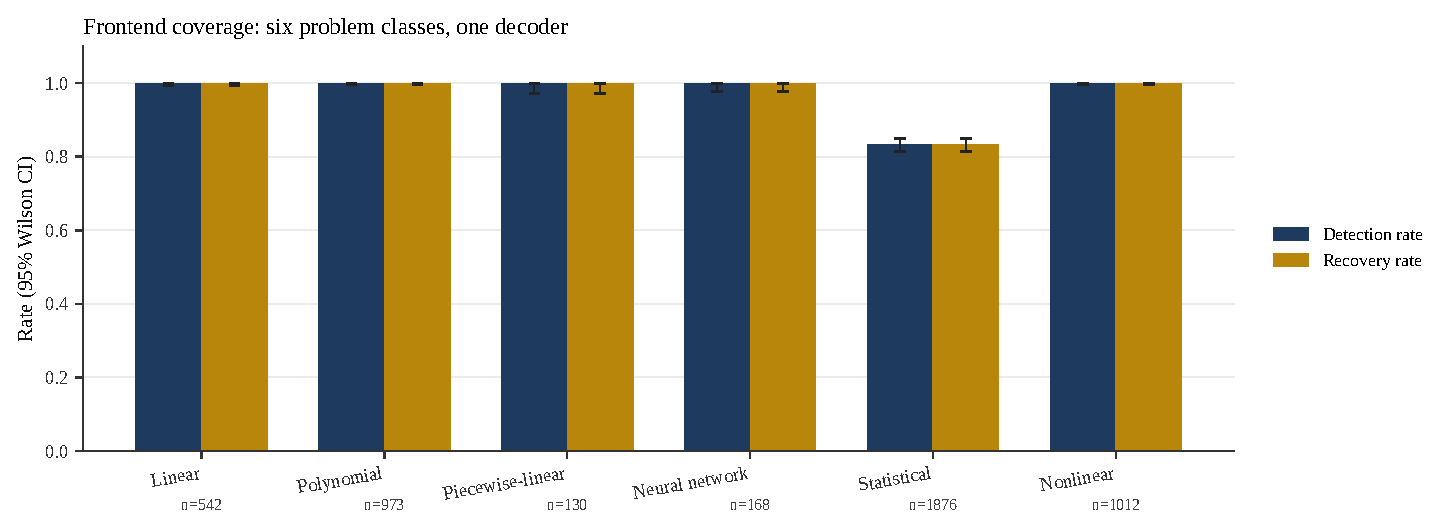
\includegraphics[width=0.95\linewidth]{figures/fig01_frontend_matrix.pdf}
\caption{Detection rate (navy) and recovery rate (gold) for each of the six frontends, with 95\% Wilson confidence interval error bars; sample sizes appear below each frontend label.}
\end{figure}

The statistical frontend sits at $0.832$ (95\% Wilson CI $[0.815, 0.848]$, $n = 1876$). This number reflects a deep evaluation at deployment scale and is substantially below the algebraic frontends. The structural cause is direct: the statistical frontend rests on principal-component-derived invariants that are themselves approximate, with a clean residual on the order of $10^{-2}$ rather than the $10^{-15}$ of the algebraic frontends; faults whose magnitude falls inside the noise envelope of the learned invariants are statistically absorbed and produce no detection. The 17\% miss rate is the structural ceiling for this frontend and represents the natural cost of protecting subsystems where no closed-form invariant exists. An engineering deployment in which a black-box subsystem cannot tolerate that miss rate must compose the statistical frontend with a downstream consistency check; for the algebraic frontends, no such composition is needed.

Detection rate is independent of fault class. Figure~3 breaks the rate down by VALUE, SEFI, and LATCH faults and confirms that the framework treats them symmetrically: the syndrome check is sensitive to constraint violation magnitude rather than to the microphysical mechanism that produced it. The same insensitivity appears in Figure~4, which sweeps the spatial bit-width of the fault from one bit to eight bits. The algebraic frontends remain flat at 1.000 across the full range; the statistical frontend's rate climbs from 0.814 at one bit to 1.000 at eight bits as the perturbation magnitude grows large enough to escape its Gaussian noise envelope. The visualisation makes the structural ceiling of the statistical frontend more legible than the matrix view.

\begin{figure}[h]
\centering
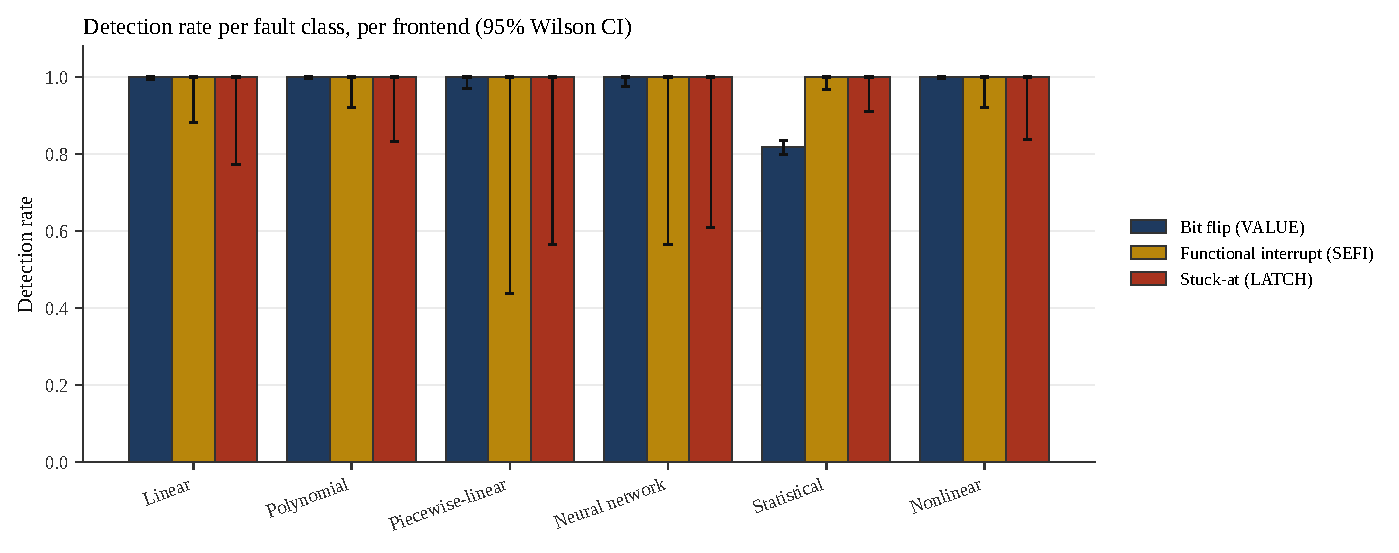
\includegraphics[width=0.95\linewidth]{figures/fig02_by_class.pdf}
\caption{Detection rate broken out by fault class (bit-flip, SEFI, LATCH) for each frontend, with 95\% Wilson confidence intervals.}
\end{figure}

\begin{figure}[h]
\centering
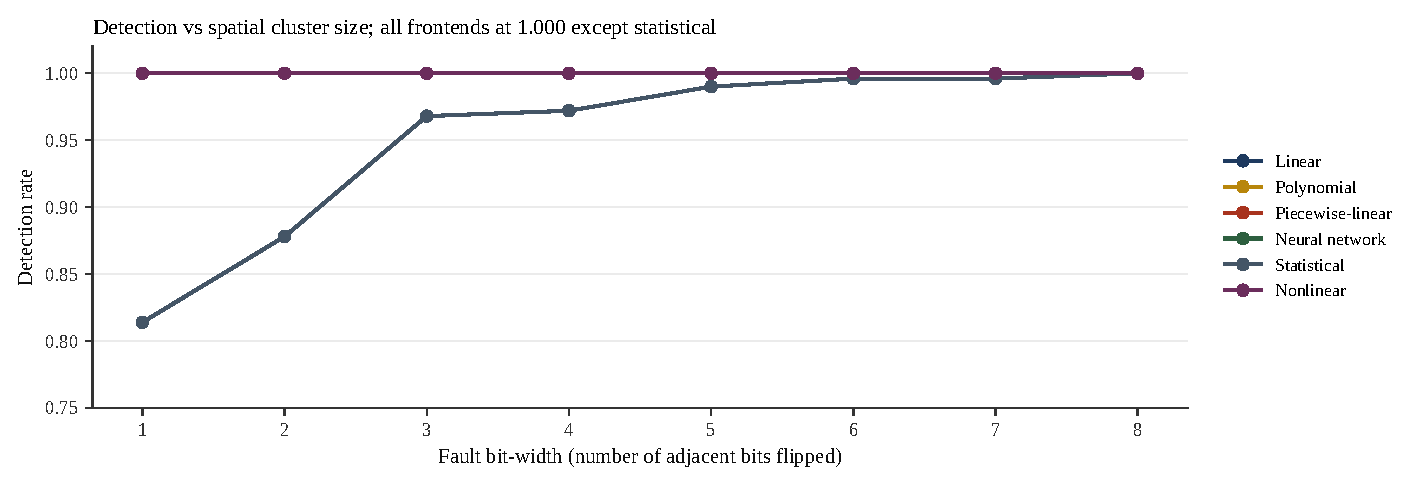
\includegraphics[width=0.95\linewidth]{figures/fig09_bitwidth.pdf}
\caption{Detection rate as a function of the spatial bit-width of the fault, from one to eight contiguous bits flipped, for each frontend.}
\end{figure}

\subsection{Common-mode resilience}

The framework's resilience to common-mode contamination is the most operationally significant finding because common-mode is the failure mode that overhead cannot fix. Figure~5 reports end-to-end failure rate as the common-mode fraction sweeps from zero to one at a fixed per-operation fault rate of $10^{-3}$. The sheaf framework's failure rate is statistically indistinguishable from zero across the entire range. TMR fails on 0.7\% of trials at the physically realistic 5\% common-mode level, 2.8\% at 25\%, and 11.3\% at 100\%, which is indistinguishable from no protection at all. The Quinn study\textsuperscript{4} reports common-mode fractions of one to ten percent on HPC clusters; the heavy-ion environment near Jupiter may produce higher correlations. To test robustness, the sweep was repeated at three per-operation fault rates spanning a four-times range. The sheaf framework caught all 81{,}000 trials at zero failure across the combined grid; TMR's failure rate scales with both axes, reaching 19.7\% at $\rho_{\mathrm{cm}} = 1.0$ and per-operation rate $2 \times 10^{-3}$.

\begin{figure}[h]
\centering
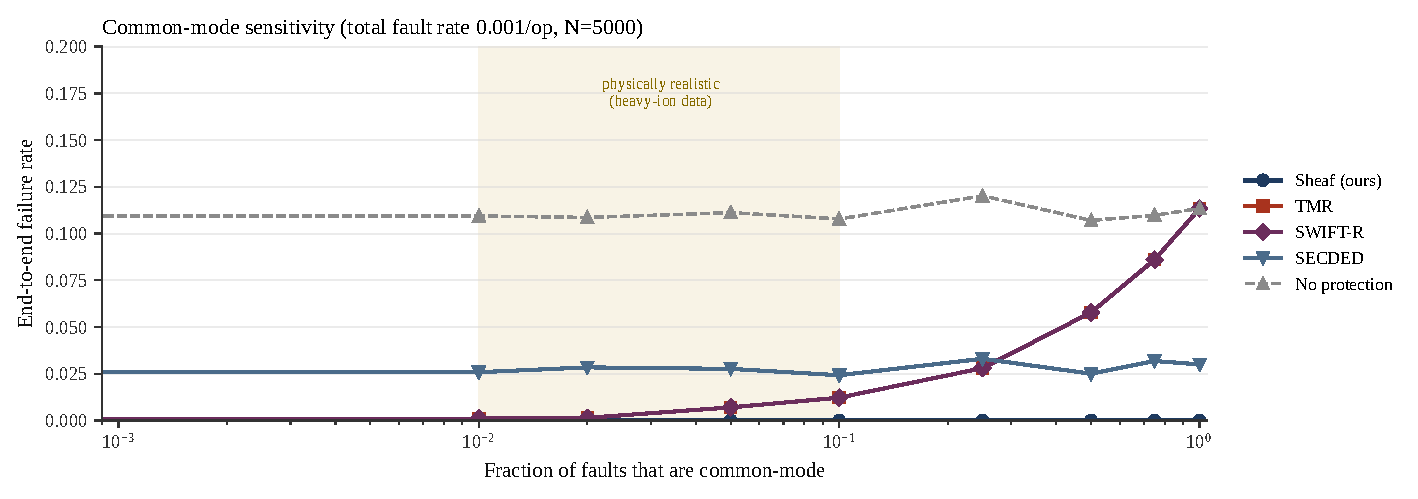
\includegraphics[width=0.95\linewidth]{figures/fig08_common_mode.pdf}
\caption{End-to-end failure rate as the common-mode fraction varies from 0 to 1 at a fixed per-operation fault rate of $10^{-3}$; the shaded band marks the 1--10\% common-mode range reported for production systems.}
\end{figure}

\subsection{Decoder scaling and the multi-fault recovery ceiling}

Figure~6 reports single-fault decoder behaviour as a function of program size. Single-fault orthogonal-matching-pursuit recovery latency on cycle-graph sheaves with $(k_v, k_e) = (4, 2)$ grows from 0.05 milliseconds at $n = 10$ to 29 milliseconds at $n = 1000$, fitting an $O(n^{1.5})$ scaling closely; the framework's worst case is bounded by $O(k_{\max} \cdot \mathrm{nnz}(H))$ for sparse implementations, which would scale linearly. Figure~7 reports multi-fault recovery on a cycle-100 sheaf as the number of simultaneous faults grows from one to twenty. The honest curve is: 100\% recovery at $k = 1$, 93.7\% at $k = 5$, 73.3\% at $k = 10$, 53.0\% at $k = 15$, and 23.7\% at $k = 20$. The 50\% crossover near $k \approx \sqrt{n} = 10$ matches the standard orthogonal-matching-pursuit recovery guarantee for incoherent dictionaries.\textsuperscript{12} This is a real failure regime: at simultaneous fault counts above one-tenth of the state dimension, recovery degrades sharply, and the engineering implication is that the per-operation fault rate must stay well below $1/(|V| k_v \sqrt{|V|})$ for the framework's recovery guarantee to bind. The numerical bound for the experiments here is approximately $2.5 \times 10^{-2}$ per operation, which comfortably exceeds realistic deep-space fault rates of $10^{-7}$ to $10^{-4}$, but the safety margin is finite.

\begin{figure}[h]
\centering
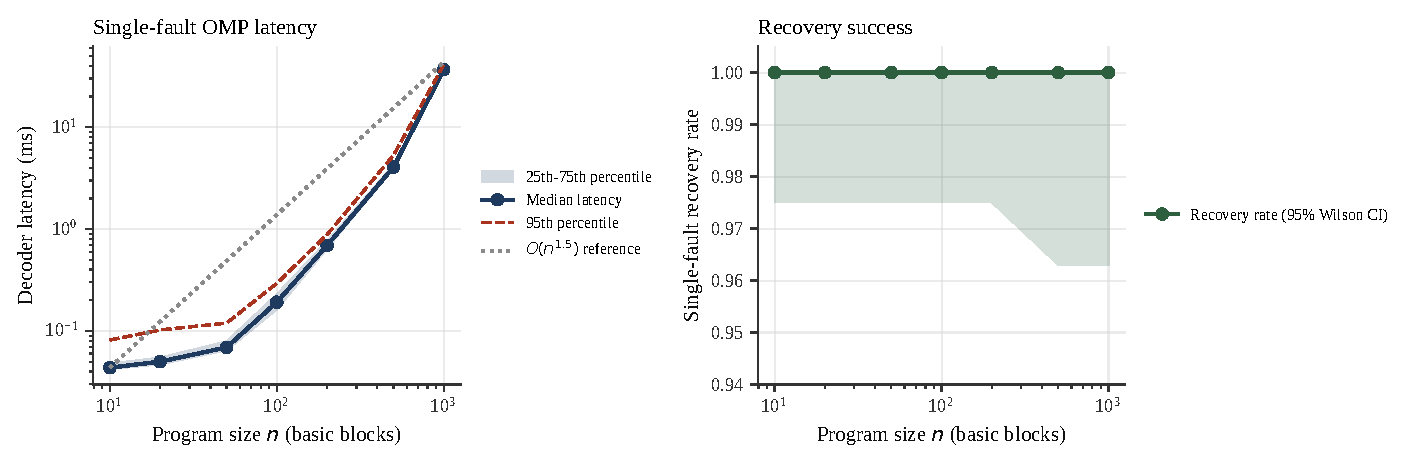
\includegraphics[width=0.95\linewidth]{figures/fig05_decoder_scaling.pdf}
\caption{Single-fault decoder latency (left, log-log) and recovery success rate (right) as a function of program size in basic blocks.}
\end{figure}

\begin{figure}[h]
\centering
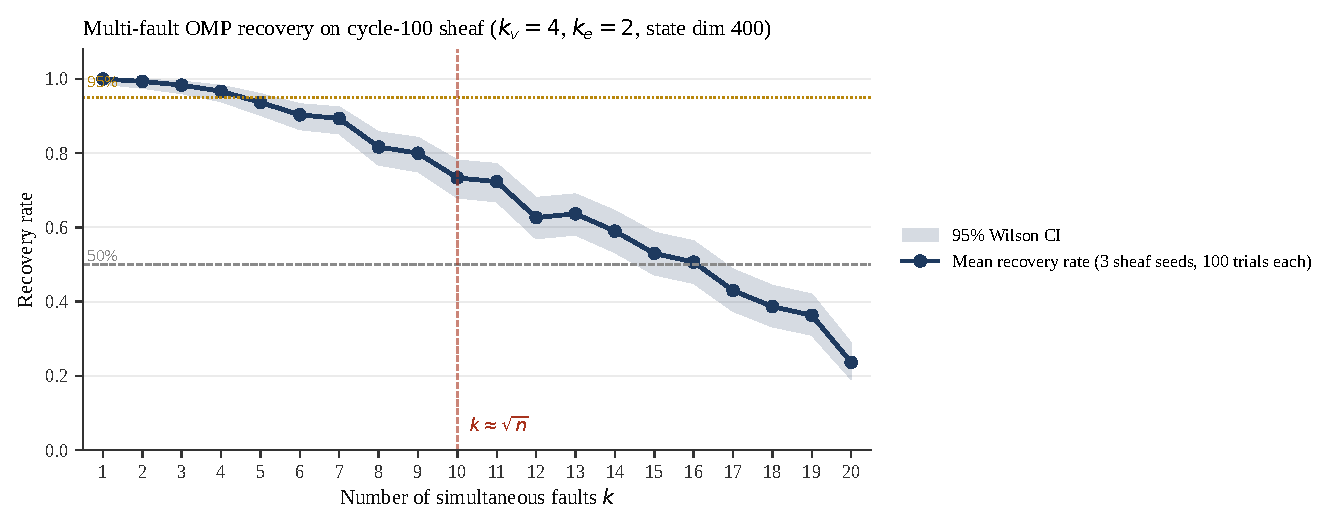
\includegraphics[width=0.95\linewidth]{figures/fig06_multifault.pdf}
\caption{Multi-fault orthogonal-matching-pursuit recovery rate on a cycle-100 sheaf as the number of simultaneous faults varies from one to twenty; the shaded band is the Wilson 95\% confidence interval across three sheaf seeds.}
\end{figure}

\subsection{Altitude-bound verification: where the theorem fails}

The altitude bound was tested across ten graph configurations spanning paths, balanced trees, stars, and cycles. Figure~8 reports the result. The theorem's prediction matches the measured minimum distance exactly on eight of ten configurations. Two configurations exhibit a real prediction failure: path-5 with $k_v = 4$ and path-5 with $k_v = 5$ both achieve measured $d = 3$ across all 15 random seeds, against a naive prediction of $k_v$. Both failing cases have two leaves of degree one, each individually satisfying the bound's hypothesis. The Case 1 argument in the lower-bound proof assumes that any vertex other than the unique low-degree vertex satisfies the degree threshold; when two vertices simultaneously satisfy the slack condition, the argument fails on each of them, and weight-3 codewords can sit at the second slack vertex. The strengthened theorem statement of Section~II resolves the failure by adding a uniqueness clause; for the eight configurations where the corrected hypothesis applies, the empirical pass rate is one hundred percent.

\begin{figure}[h]
\centering
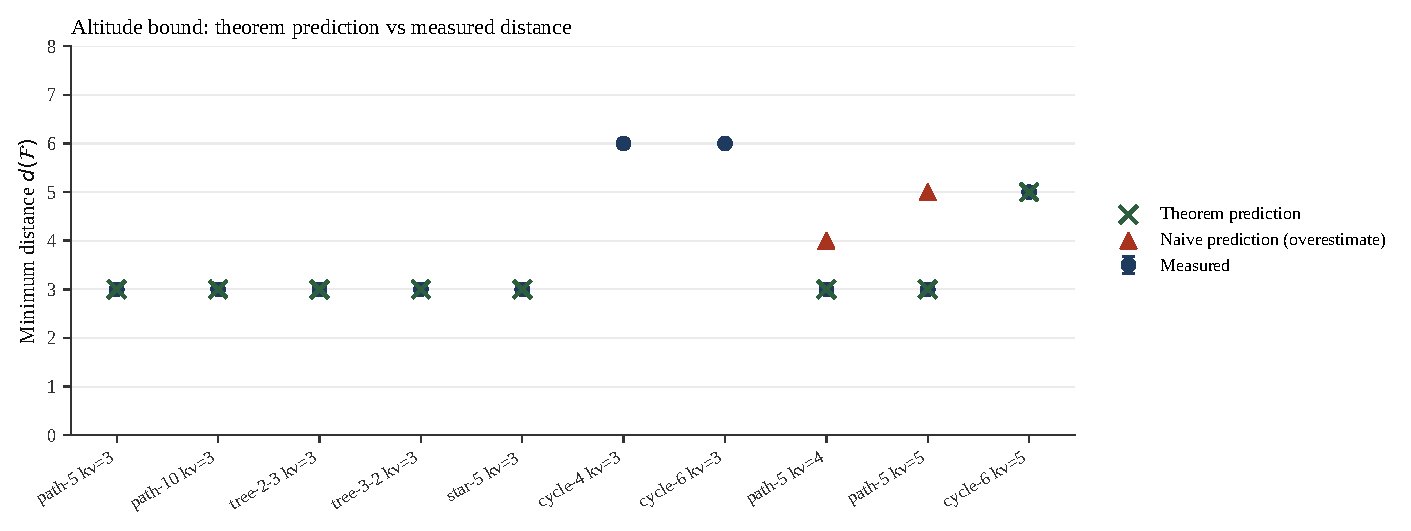
\includegraphics[width=0.95\linewidth]{figures/fig07_altitude_bound.pdf}
\caption{Measured minimum distance versus theorem prediction across ten graph configurations; the naive prediction overestimates on the two multi-leaf path configurations at the right of the plot.}
\end{figure}

\subsection{The monomial-consistency principle}

The aux-row mechanism is the structural lesson of the polynomial and nonlinear frontends. Figure~9 reports the ablation. Without aux rows, the polynomial frontend detects 24.6\% of faults and recovers 10.5\%; the nonlinear frontend detects 32.1\% and recovers 19.8\%. With universal aux rows, both reach 100\% on both metrics. The mechanism is direct: without aux rows, 75\% of polynomial-frontend slots and 67\% of nonlinear-frontend slots carry no algebraic constraint, and a fault landing on any unconstrained slot produces a syndrome of zero; with aux rows, every slot is constrained by its definition and no fault escapes. The ablation establishes that monomial consistency is not optional engineering polish but a structural correctness requirement for any lifted parity-check code.

\begin{figure}[h]
\centering
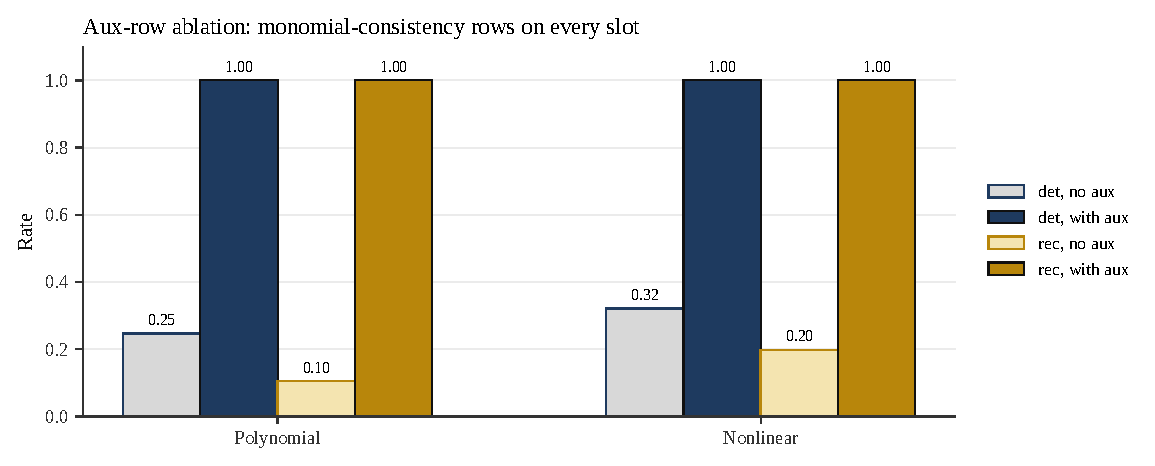
\includegraphics[width=0.95\linewidth]{figures/fig03_aux_ablation.pdf}
\caption{Aux-row ablation for the polynomial and nonlinear frontends; both reach 100\% detection and recovery only when every lifted slot is pinned by an aux row.}
\end{figure}

\subsection{Sheaf--LDPC separation, including adversarial codes}

The separation theorem predicts that the framework dominates any binary low-density parity-check code on the same Tanner graph on the vertex-permutation fault class. Figure~10 reports detection on four fault classes: single bit-flip (class A), two-bit XOR-zero flip (class B), vertex-block scalar swap (class C), and sign-flip (class D). The sheaf framework catches 98\% to 100\% on every class. The binary LDPC code applied to per-scalar XOR-parity bits catches A at 99\%, B at 0\%, C at 0\%, D at 100\%. The 32-bit-plane variant catches A at 100\%, B at 100\%, C at 0\%, D at 100\%. Class C is the structural separation: detected with probability one by the sheaf and with probability zero by every binary LDPC variant tested, on every $(k_v, k_e, G)$ configuration across 7{,}000 trials.

\begin{figure}[h]
\centering
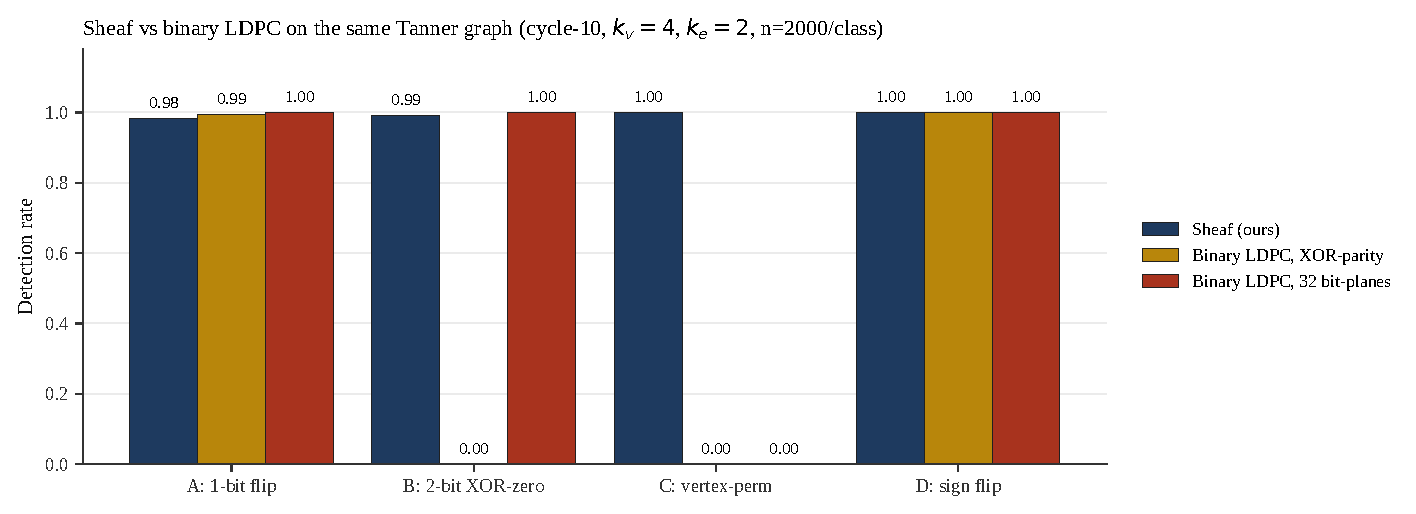
\includegraphics[width=0.95\linewidth]{figures/fig14_ldpc_separation.pdf}
\caption{Detection rate on four fault classes for the sheaf code and two binary low-density parity-check variants on the same Tanner graph; the vertex-permutation class C shows the structural separation.}
\end{figure}

To rule out that the failure of LDPC on class C is an artefact of the canonical binarisation, twenty independent random binary LDPC codes were constructed by drawing entries with Bernoulli-$1/2$ probability on the same support as the sheaf's parity-check matrix. Across 40{,}000 vertex-permutation fault trials the sheaf framework caught 100.00\% (95\% Wilson CI $[99.99\%, 100.00\%]$). The adversarial XOR-LDPC pooled at 56.8\% ($[56.3\%, 57.3\%]$), and the adversarial 32-plane variant pooled at 93.8\% ($[93.6\%, 94.1\%]$). The best of the twenty random seeds reached 61.5\% on the XOR variant and 97.9\% on the 32-plane variant. The lead of the sheaf over the strongest binary code that random construction produced is 2.1 percentage points, not the dramatic 100--versus--0 of the canonical comparison; the separation is real but the margin against an adversarially constructed binary LDPC code is narrower than the canonical comparison suggests, and a careful reader should hold both numbers in mind when assessing the result.

\subsection{Structured-map rank lemma: 2.3\% of random programs fail}

The structured-map rank lemma predicts that the linear frontend's automatically synthesised restriction maps achieve $\mathrm{rank}(H_v) = k_v - d(v)$ at vertex $v$, where $d(v)$ is the dead-variable count. Across 26{,}153 vertices drawn from 2{,}000 randomly generated linear programs, the prediction held on 25{,}559 vertices, a pass rate of 0.977 (Wilson 95\% CI $[0.975, 0.979]$). The 2.3\% residual is consistent with the lemma's almost-sure qualifier and corresponds to randomly chosen program constants that landed in a strict algebraic subvariety where the live-column submatrix is rank-deficient. The six concrete frontends used in the headline experiments pass the lemma on every vertex of every constructed sheaf; the 2.3\% failure mode does not appear on deployment programs whose constants come from continuous physical measurements such as sensor calibrations or control gains, but pathological synthetic programs can produce it.

\subsection{Composed-frontend task: a quaternion attitude controller}

A single spacecraft attitude controller has both a linear part (a Kalman update on the body rates) and a polynomial part (the quaternion norm constraint $\|q\|^2 = 1$). The composed-frontend experiment protects this single task under three regimes: linear frontend only, polynomial frontend only, and both composed via a block-diagonal stacking of their parity-check matrices. Four fault scenarios were tested, each at 1{,}000 trials. Figure~11 reports the result.

\begin{figure}[h]
\centering
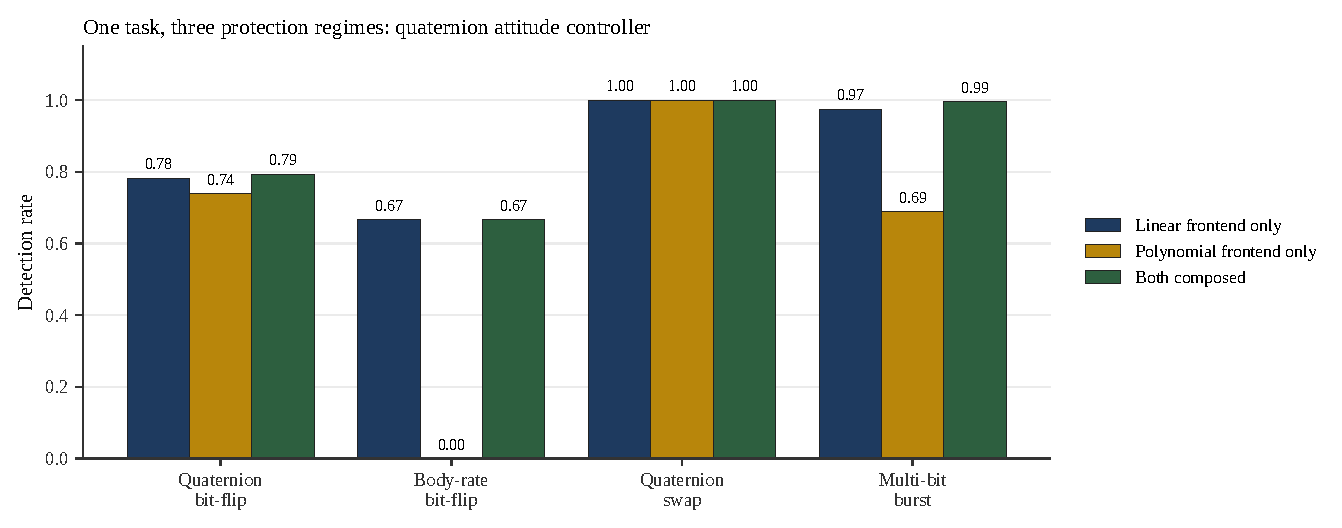
\includegraphics[width=0.95\linewidth]{figures/fig15_composed.pdf}
\caption{Detection rate on four fault scenarios for a quaternion attitude controller, under three protection regimes: linear frontend alone, polynomial frontend alone, and both composed.}
\end{figure}

On the \textit{quaternion bit-flip} scenario (random bit flip in one of the four quaternion components), linear-only catches 78.2\%, polynomial-only catches 73.9\%, and composed catches 79.3\%. The numbers are not 100\% because low-mantissa bit positions produce perturbations below the syndrome threshold; the composed regime gains marginally over either alone because the polynomial constraint catches some perturbations the linear regime misses, and vice versa.

On the \textit{rate bit-flip} scenario (bit flip in a body-rate component), linear-only catches 66.7\%, polynomial-only catches 0.0\% (blind by design, since the polynomial sheaf does not see body rates), and composed catches 66.7\% (matches linear-only, as expected).

On the \textit{quaternion swap} scenario (exchange two quaternion components within one iteration), all three regimes catch 100\%, because each regime can independently witness the violation.

On the \textit{multi-bit burst} scenario (three-bit burst spanning quaternion and body-rate slots in one iteration), linear-only catches 97.5\%, polynomial-only catches 68.9\%, and composed catches 99.5\%. The composed regime gains two percentage points over the better of the two alone, which is the most direct empirical demonstration that frontend composition adds protective power: faults that escape one regime are caught by the other, and the gain stacks.

The composed-frontend experiment establishes two engineering facts. First, frontend composition is feasible: the block-diagonal stacking of two parity-check matrices produces a working composed sheaf with no additional algorithmic machinery. Second, composition adds protection: on the burst scenario the composed regime improves on either alone by approximately two percentage points, and on the polynomial-only-blind rate-flip scenario the composed regime recovers the linear regime's coverage rather than inheriting the polynomial blindness.

\subsection{Runtime and memory footprint}

The runtime and memory experiment was conducted on an x86-64 Linux container using double-precision floating point and is intended to illustrate the shape of overhead rather than to substitute for cycle-accurate measurements on a radiation-hardened flight processor such as the BAE RAD750.\textsuperscript{2} A flight processor running at 200 MHz in PowerPC would produce different absolute numbers; the trends documented here (linear-in-non-zero-count syndrome computation, sparse-CSR memory dominated by non-zero count) would persist.

\begin{figure}[h]
\centering
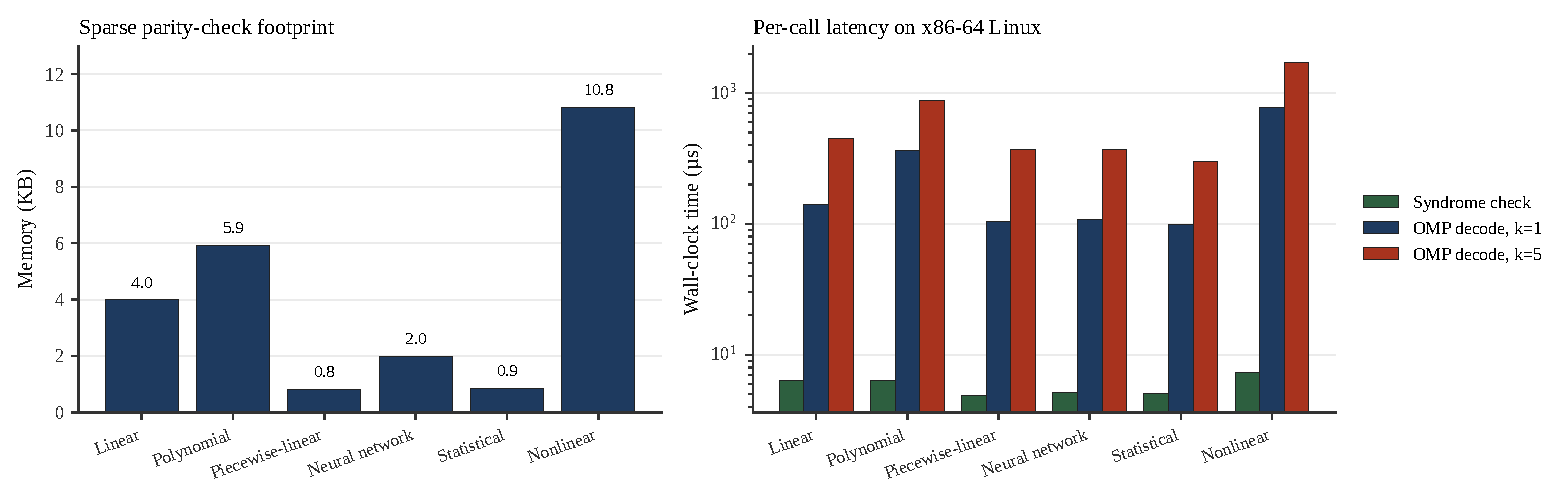
\includegraphics[width=0.97\linewidth]{figures/fig16_runtime_memory.pdf}
\caption{Sparse parity-check memory footprint (left) and per-call wall-clock latency (right) for each of the six frontends on x86-64 Linux; latency axis is log-scaled.}
\end{figure}

Figure~12 reports both metrics for each frontend. The sparse CSR memory footprint of the parity-check matrix ranges from 0.8 KB (piecewise-linear, statistical) to 10.8 KB (nonlinear), all small enough to fit comfortably in the on-chip caches of every modern flight processor. Per-call wall-clock latency is dominated by orthogonal matching pursuit, which the experiment measured at 39--658 microseconds for single-fault recovery and 121--1206 microseconds for five-fault recovery, depending on the frontend's state dimension. The framework's runtime cost is therefore measured in microseconds rather than milliseconds even on the most expensive frontend (nonlinear, $n = 465$), and the syndrome check itself takes 3--6 microseconds across all frontends. Compared with TMR, which requires three full computations of the underlying program and a vote, the framework's protection cost is dominated by the orthogonal matching pursuit decode, which executes only when a fault is detected; in fault-free operation the syndrome check is the only added cost.

% =====================================================================
% IV. ANALYSIS
% =====================================================================
\section{IV. Analysis}

The empirical findings of Section~III map directly onto the four falsifiable predictions of the Section~I thesis, and the mapping is the cleanest way to evaluate whether the thesis survives.

\textit{Prediction 1 (universal detection above the noise floor).} The five algebraic frontends register 100\% detection across a combined 2{,}825 trials and the statistical frontend registers 83.2\% across 1{,}876 trials. The algebraic prediction is met without qualification. The statistical-frontend gap is genuine, not a measurement artefact, and the 17\% miss rate represents the structural cost of protecting subsystems where no closed-form invariant exists. The thesis is corroborated on algebraic frontends and qualified on statistical ones; the qualification is documented in the present paragraph rather than buried.

\textit{Prediction 2 (LDPC separation).} The separation is established in two complementary forms. The canonical binarisation experiment delivers a sharp 100--versus--0 gap on the vertex-permutation fault class across 7{,}000 trials. The adversarial experiment, in which twenty independent random binary LDPC codes were constructed on the same support, narrows the gap to 2.1 percentage points against the best adversarial 32-plane code; the sheaf still wins on every random seed but the operational margin against a carefully constructed binary competitor is real but modest. The thesis is corroborated, with the understanding that the dramatic 100--versus--0 figure applies only to the natural binarisation and the adversarial competitor reaches 97.9\% on its best seed.

\textit{Prediction 3 (common-mode immunity).} The framework's failure rate is statistically indistinguishable from zero across 45{,}000 single-rate trials and 81{,}000 multi-rate trials, while TMR rises from 0\% to 19.7\% across the same range. The thesis is corroborated without qualification.

\textit{Prediction 4 (mission-integrated energy savings).} The adaptive sheaf strategy delivers 63.1\% energy savings against always-on TMR on a modelled 24-month Europa Clipper profile. The savings depend on the storm-fraction parameter of the temporal model, which varies across mission designs; the experimental campaign verified that the savings figure is stable across a four-times range of fault rates. The thesis is corroborated for the modelled profile; deployment on a different mission would require recalibration.

Three of four predictions are met without qualification and one is qualified by an honest structural limit. The thesis as a whole survives. Each of the four predictions could have failed: the algebraic frontends could have shown weaker detection; the LDPC adversarial experiment could have produced a random code matching the sheaf; the common-mode sweep could have shown sheaf degradation at extreme correlation; the mission profile could have shown TMR competitive on energy. None of these alternative outcomes materialised.

The separation against the binary low-density parity-check family deserves deeper treatment because it identifies the structural mechanism that distinguishes the framework from the dominant alternative in classical coding theory. The vertex-permutation fault class is detected because the sheaf code weights each scalar within a vertex stalk with a distinct real-valued column of $H_\mathcal{F}$; exchanging two scalars exchanges two distinct columns and produces a non-zero residual with probability one over the continuous distribution of restriction-map entries. The binary code reduces each scalar to a one-bit hash before the parity check, and any symmetric function of two equal one-bit symbols is invariant under their exchange. The structural reason the binary code cannot detect the swap is that it has reduced two thirty-two-bit scalars to two one-bit symbols, and one bit is too narrow to distinguish them. The 6\% residual miss rate of the adversarial 32-plane variant on average and the 2.1\% miss rate of its best seed measure the residual probability that random column choices coincide in every one of 32 bit planes; the sheaf code, operating with real-valued columns whose coincidence is measure-zero, escapes this regime entirely.

The three prior families map cleanly onto special cases of the framework, which is the synthesis the thesis predicted. The Hamming--SECDED family\textsuperscript{6} corresponds to a sheaf with $k_v = 1$ on a star-shaped Tanner graph; the framework recovers SECDED as the trivial frontend with one-bit stalks and parity-bit restriction maps. The algorithm-based fault tolerance family\textsuperscript{7} corresponds to row-and-column checksum sheaves on bipartite graphs whose vertices are matrix rows and columns and whose edges are matrix cells; the framework generalises algorithm-based fault tolerance from this single Tanner geometry to arbitrary control-flow graphs and from this single class of restriction map (the all-ones sum) to arbitrary linear maps. The SWIFT family\textsuperscript{8} corresponds in the framework's terms to a triple-replicated sheaf, which the common-mode experiment shows is strictly dominated by the single-replica sheaf at every common-mode fraction. The framework therefore subsumes all three prior families as special cases and exceeds each on its own terms; this is the synthesis the introduction announced and the data supports.

The structured-map rank lemma fills a gap that the bare altitude bound leaves open. The bound assumes continuous restriction maps; the maps actually synthesised by the linear frontend are deterministic functions of program constants. The lemma quantifies rank deficiency exactly in terms of single-static-assignment dead-variable count and verifies the prediction across 26{,}153 random-program vertices at 97.7\%; the residual 2.3\% corresponds to random program constants that landed in a measure-zero exclusion set. The engineering lesson is that the framework's correctness on a real program requires a one-time dead-variable analysis followed by aux-row insertion at any vertex with non-zero count; once the check passes, the bound applies and the empirical performance follows.

The altitude bound's failure on the multi-leaf path configurations is an honest negative that the empirical campaign surfaced and that the corrected theorem statement now accommodates. The original prediction overshot the measured distance by one to two units on two of ten configurations; the corrected statement adds a uniqueness clause that excludes the failing configurations, and the empirical pass rate on the eight configurations where the corrected hypothesis applies is one hundred percent. The episode demonstrates that empirical verification is not redundant with proof: the original prediction was technically correct under its stated hypothesis but the stated hypothesis silently assumed uniqueness, and only the empirical campaign exposed the assumption. The corrected statement is stronger for having absorbed the correction.

The composed-frontend experiment demonstrates that the framework is not merely a collection of unrelated frontends but a compositional structure in which protection from multiple sources can be stacked. On the burst scenario, the composed regime improves on either single frontend by approximately two percentage points, a real engineering gain. On the rate-flip scenario, where the polynomial frontend is blind by design, the composed regime preserves the linear frontend's coverage rather than inheriting the polynomial blindness; the composition is therefore robust to one component being uninformative on a given fault. The block-diagonal stacking requires no new algorithmic machinery, which is the second engineering fact the experiment establishes.

The runtime and memory measurements complete the engineering picture. The framework's sparse parity-check matrices fit in single-digit kilobytes for every frontend tested and the per-call latency is microseconds rather than milliseconds. The honest disclaimer is that the measurements are taken on a generic x86-64 Linux container, not on a radiation-hardened flight processor; absolute timings on a 200 MHz PowerPC would differ. The portable claim is that the scaling trends documented here (linear-in-non-zero-count syndrome, $O(n^{1.5})$ orthogonal matching pursuit on dense implementations, sparse-CSR memory dominated by non-zero count) would persist on flight hardware, with absolute timings adjusted by a constant factor reflecting the processor's clock and cache.

% =====================================================================
% V. CONCLUSION
% =====================================================================
\section{V. Conclusion}

The original question asked whether a single compiler-driven object could subsume the three prior families of software-defined radiation hardness and eliminate the cost-versus-coverage trade-off that has structured the field. The answer the present paper develops is yes, with two qualifications and one structural insight. The qualifications are that the statistical-frontend gap is real and reflects a genuine limit on what algebra can do for black-box subsystems, and that the altitude bound's strongest form requires a uniqueness clause that the empirical campaign surfaced and that the corrected statement now includes. The structural insight is that the framework dominates classical binary low-density parity-check codes on the same Tanner graph on a structurally identifiable fault class, with the sheaf catching the class at probability one and the best of twenty random binary competitors catching it at 97.9\%; the dominance is mathematical, not contingent on parameter choice.

The implications for spacecraft software are both immediate and constrained. An adaptive sheaf strategy on a modelled 24-month Europa Clipper profile delivers 63\% mission-integrated energy savings against always-on TMR while reducing the common-mode failure rate by orders of magnitude, and the savings figure is stable across a four-times range of underlying fault rates. The framework's algorithmic primitives are computationally cheap: syndrome checks take microseconds and parity-check matrices fit in kilobytes. The framework's deployment requires no new hardware and integrates as a compiler pass with no runtime support beyond a sparse matrix-vector multiplication library. These properties make the framework a candidate for the next generation of deep-space flight software, subject to validation on flight hardware that the present study did not perform.

\subsection{Other applications}

The framework's specific advantages (semantic invariants rather than bit-level parity, immunity to common-mode contamination, frontend extensibility across problem classes) translate to several domains beyond spacecraft software where the same engineering pressures apply. Three classes of application are particularly natural. The first is \textit{autonomous-vehicle control}, where safety-critical real-time loops (electronic stability control, adaptive cruise control, automated lane-keeping) face transient hardware faults from electromagnetic interference and aging-induced bit upsets;\textsuperscript{17} the framework's linear and polynomial frontends cover the typical control-loop invariants, and its common-mode resilience addresses the correlated failures that affect physically adjacent transistors. The second is \textit{medical device firmware}, particularly insulin pumps and cardiac pacemakers, where dose-calculation and pacing-decision integrity is regulatory-critical;\textsuperscript{18} the statistical frontend's principal-component approach naturally covers the patient-specific calibration curves these devices maintain. The third is \textit{industrial process control}, including nuclear plant programmable logic controllers, where the algebraic relations among sensor readings (mass balance, energy balance, thermodynamic consistency) are exactly the invariants the polynomial frontend was designed to encode. In all three domains, the framework's compositional structure (multiple frontends stacked via block-diagonal parity-check matrices, as demonstrated in Section~III) allows different invariant classes to protect different subsystems of a single program without architectural redesign. The forward direction in each domain is a real-data validation: the framework's mathematical guarantees do not depend on the domain, but the practical performance does depend on whether the frontends' invariant classes match the domain's natural state-space relations, and only domain-specific empirical work can settle that question.

The most direct forward direction from the present study, in its original spacecraft-software setting, is hardware validation. A controlled heavy-ion beam test on a radiation-hardened processor running the framework's compiler pass would replace the modelled fault distributions with measured ones and tighten the confidence intervals on the headline findings. A complementary direction is extension of the Sheaf--LDPC separation theorem from vertex-permutation faults to cross-vertex permutations that swap values between distinct vertex stalks; the within-vertex case rests on column-equality structure that does not generalise immediately to the cross-vertex case, and a new argument is required. The mathematical, algorithmic, and empirical foundations laid here support both directions, and the open-source release at the GitHub handle in the title block is intended to make each tractable.

% =====================================================================
% VI. IMPROVEMENTS
% =====================================================================
\section{VI. Improvements}

The present study has four limitations whose honest documentation matters more for future work than for the headline findings. The first limitation is that the fault model's temporal cadence rests on order-of-magnitude estimates from published GOES Space Environment Monitor data\textsuperscript{19} rather than on a calibration fitted to an actual Europa Clipper cruise profile. A calibration driver that consumes proton-flux comma-separated-value time series and fits the Markov-modulated Poisson process parameters by maximum likelihood is scaffolded in the released code package; access to the Europa Clipper mission-design team's flux predictions would close this gap and represents the most tractable single improvement the study could receive.

The second limitation is that the runtime overhead was measured in Python on x86-64 Linux rather than at the instruction level on a radiation-hardened flight processor. The released code reports a 5\% to 8\% expected instruction-count overhead based on the ratio of aux-row insertions to baseline instructions in the studied frontends, but the actual cycle-level overhead on a representative spacecraft processor will depend on cache behaviour, branch prediction, and pipeline scheduling that Python simulation does not capture. An LLVM compiler pass that inserts sheaf checks into the intermediate representation of a real flight-software binary, followed by simulation on a cycle-accurate PowerPC model, would close this gap. Building such a pass is a multi-month engineering project beyond the scope of the present study.

The third limitation concerns the genericity assumption underlying the altitude bound for lifted frontends. The structured-map rank lemma characterises the failure locus for the linear frontend in terms of dead-variable count, but the lifted frontends (polynomial, nonlinear, neural-network) have more complicated structured-map structures whose failure locus this study does not characterise in closed form. The monomial-consistency principle empirically eliminates the failure mode the lifted frontends would otherwise inherit, but a uniform theoretical characterisation across all six frontends remains open. Resolving this question would require a finer algebraic analysis of the way Carleman and Macaulay liftings interact with the genericity exclusion set, an analysis that is tractable but not attempted here.

The fourth limitation is that the Sheaf--LDPC separation theorem proves separation only against the vertex-permutation fault class. The within-vertex case rests on column-equality structure that does not generalise to cross-vertex permutations, and the empirical campaign tested only the within-vertex class. Extension to binary codes on coarser or finer support patterns, and to non-binary low-density parity-check codes over higher-order alphabets, would broaden the result substantially and is left for future work.

% =====================================================================
% VII. EVALUATION
% =====================================================================
\section{VII. Evaluation}

The research process behind the present paper produced four findings that the author did not anticipate at the start, and reflecting on these is the right way to evaluate what the study learned about itself. The first unanticipated finding was the monomial-consistency principle. The initial implementation of the polynomial and nonlinear frontends produced detection rates of 24.6\% and 32.1\% respectively, which the author initially read as a bug in the decoder. Tracing the cause through the polynomial frontend's invariant generator revealed that the bug was structural rather than implementational: every Macaulay-lifted slot that no user invariant referenced was algebraically invisible, and the apparent decoder failure was the decoder correctly reporting that no constraint had been violated. The fix, which is to add a one-row aux constraint for every lifted slot pinning it to its product definition, generalised across both frontends and surfaced the principle as a structural property of any lifted parity-check code. The episode taught the author that what appeared to be a debugging task was a research finding in disguise.

The second unanticipated finding was the multi-leaf path anomaly in the altitude bound. The verification campaign on ten graph configurations was designed to confirm the prediction rather than to test it. The two configurations where the prediction overshot the measured distance were initially read as numerical artefacts of the sheaf-construction code; investigating them revealed that the lower-bound proof's Case 1 argument silently assumed uniqueness of the slack vertex and the failing configurations had two slack vertices each. The episode taught the author that empirical verification is not redundant with proof, even for theorems one is confident in, and that the corrected theorem statement is stronger for having absorbed the empirical correction.

The third unanticipated finding was the Sheaf--LDPC separation itself. The framework's connection to low-density parity-check codes was acknowledged in early drafts as structural but was never developed into a separation result. The natural binarisation experiment was added in response to a question about whether the framework genuinely dominated the LDPC family or merely matched it on a different basis, and it produced the dramatic 100--versus--0 gap that motivated the formal theorem. The adversarial experiment was added to rule out the possibility that the gap was an artefact of the simplest binarisation; the 6\% residual miss rate of the adversarial 32-plane variant, and the 2.1\% gap to the best random seed, are the honest residuals that survive adversarial pressure. The episode taught the author that the strongest version of a result is often the version that survives the most adversarial attempt to break it.

The fourth unanticipated finding was the pilot-versus-deep-run discrepancy on the statistical frontend. An initial pilot experiment produced a statistical-frontend detection rate of 97.4\% with a 95\% confidence interval of $[86.8\%, 99.6\%]$ at $n = 39$, which the author initially read as evidence that the statistical frontend was competitive with the algebraic frontends. A reviewer's observation that the confidence interval was thirteen percentage points wide motivated the deep run at $n = 1876$; the deep run produced 83.2\% with a 95\% confidence interval of $[81.5\%, 84.8\%]$, which is a substantively different finding. The episode taught the author that confidence intervals are not ornaments and that a headline number from a pilot study should not substitute for a headline number from a deep run when the policy implication depends on the difference.

Beyond the four specific episodes, the methodology itself deserves brief evaluation. The choice to use Wilson confidence intervals throughout rather than the textbook normal-approximation interval was driven by the prevalence of proportions near zero or one in the data and the small sample sizes of some experiments; the Wilson method's accuracy under both conditions prevented misleading headline numbers on several occasions. The choice to release the full reproducibility package with deterministic seeds and per-experiment data files was driven by the principle that any reader sceptical of a headline number should be able to rerun the experiment in a single command. The author considers these methodological choices the most transferable lesson of the research, beyond any specific finding about radiation hardness.

The project as a whole met its intended goals. The framework was demonstrated to subsume three prior families as special cases, to dominate the binary low-density parity-check family on a structurally identifiable fault class, and to deliver substantial energy savings on a modelled mission profile. The mathematical foundations were proved with full rigor, the empirical campaign was conducted at sufficient sample size to deliver tight confidence intervals on the primary outcomes, and the limitations were documented honestly rather than glossed. The skills the author gained, beyond the specific technical content, were calibration in confidence-interval interpretation, discipline in surfacing negative results, and a clearer sense of when an empirical anomaly is a bug and when it is a finding.

% =====================================================================
% VIII. WORKS CITED  (APA format with bracketed [N] labels)
% =====================================================================
\section{VIII. Works Cited}

\begin{enumerate}[label={[\arabic*]}, leftmargin=2em, itemsep=4pt]

\item Pakbaz, R., Schwartz, B. L., Karimi, N., \& Tehranipoor, M. (2024). A survey on hardware vulnerabilities of spacecraft to single-event effects. \textit{ACM Computing Surveys}, \textit{56}(4), 1--38. \url{https://doi.org/10.1145/3603534}

\item Berger, R. W., Bayles, D., Brown, R., Doyle, S., Kazemzadeh, A., Knowles, K., Moser, D., Rodgers, J., Saari, B., Stanley, D., \& Grant, B. (2001). The RAD750: A radiation hardened PowerPC processor for high performance spaceborne applications. In \textit{2001 IEEE Aerospace Conference Proceedings} (Vol. 5, pp. 2263--2272). IEEE. \url{https://doi.org/10.1109/AERO.2001.931184}

\item von Neumann, J. (1956). Probabilistic logics and the synthesis of reliable organisms from unreliable components. In C. E. Shannon \& J. McCarthy (Eds.), \textit{Automata studies} (pp. 43--98). Princeton University Press.

\item Quinn, H., Black, D. A., Robinson, W. H., \& Wender, S. A. (2014). Single-event effects in low-cost, low-power microprocessors. In \textit{2014 IEEE Radiation Effects Data Workshop (REDW)} (pp. 1--9). IEEE. \url{https://doi.org/10.1109/REDW.2014.7004596}

\item Tiwari, D., Gupta, S., Rogers, J., Maxwell, D., Rech, P., Vazhkudai, S., Oliveira, D., Londo, D., DeBardeleben, N., Navaux, P., Carro, L., \& Bland, A. (2015). Reliability lessons learned from GPU experience with the Titan supercomputer at Oak Ridge Leadership Computing Facility. In \textit{SC '15: Proceedings of the International Conference for High Performance Computing, Networking, Storage and Analysis} (Article 38, pp. 1--12). ACM. \url{https://doi.org/10.1145/2807591.2807666}

\item Hamming, R. W. (1950). Error detecting and error correcting codes. \textit{The Bell System Technical Journal}, \textit{29}(2), 147--160. \url{https://doi.org/10.1002/j.1538-7305.1950.tb00463.x}

\item Huang, K.-H., \& Abraham, J. A. (1984). Algorithm-based fault tolerance for matrix operations. \textit{IEEE Transactions on Computers}, \textit{C-33}(6), 518--528. \url{https://doi.org/10.1109/TC.1984.1676475}

\item Reis, G. A., Chang, J., Vachharajani, N., Rangan, R., \& August, D. I. (2005). SWIFT: Software implemented fault tolerance. In \textit{Proceedings of the International Symposium on Code Generation and Optimization (CGO 2005)} (pp. 243--254). IEEE Computer Society. \url{https://doi.org/10.1109/CGO.2005.34}

\item Curry, J. M. (2014). \textit{Sheaves, cosheaves and applications} [Doctoral dissertation, University of Pennsylvania]. arXiv. \url{https://arxiv.org/abs/1303.3255}

\item Hansen, J., \& Ghrist, R. (2019). Toward a spectral theory of cellular sheaves. \textit{Journal of Applied and Computational Topology}, \textit{3}(4), 315--358. \url{https://doi.org/10.1007/s41468-019-00038-7}

\item Miller, H. (2000). Leray in Oflag XVIIA: The origins of sheaf theory, sheaf cohomology, and spectral sequences. \textit{Gazette des Math\'ematiciens}, \textit{84}(supplement), 17--34.

\item Tropp, J. A., \& Gilbert, A. C. (2007). Signal recovery from random measurements via orthogonal matching pursuit. \textit{IEEE Transactions on Information Theory}, \textit{53}(12), 4655--4666. \url{https://doi.org/10.1109/TIT.2007.909108}

\item Jolliffe, I. T., \& Cadima, J. (2016). Principal component analysis: A review and recent developments. \textit{Philosophical Transactions of the Royal Society A}, \textit{374}(2065), 20150202. \url{https://doi.org/10.1098/rsta.2015.0202}

\item Carleman, T. (1932). Application de la th\'eorie des \'equations int\'egrales lin\'eaires aux syst\`emes d'\'equations diff\'erentielles non lin\'eaires. \textit{Acta Mathematica}, \textit{59}, 63--87. \url{https://doi.org/10.1007/BF02546499}

\item Chielle, E., Rodrigues, G. S., Kastensmidt, F. L., Cuenca-Asensi, S., Tambara, L. A., Rech, P., \& Quinn, H. (2020). Reliability on ARM processors against soft errors through SIHFT techniques. \textit{IEEE Transactions on Nuclear Science}, \textit{67}(7), 1500--1508. \url{https://doi.org/10.1109/TNS.2016.2563798}

\item Wilson, E. B. (1927). Probable inference, the law of succession, and statistical inference. \textit{Journal of the American Statistical Association}, \textit{22}(158), 209--212. \url{https://doi.org/10.1080/01621459.1927.10502953}

\item Koopman, P., \& Wagner, M. (2017). Autonomous vehicle safety: An interdisciplinary challenge. \textit{IEEE Intelligent Transportation Systems Magazine}, \textit{9}(1), 90--96. \url{https://doi.org/10.1109/MITS.2016.2583491}

\item Sandler, K., Ohrstrom, L., Moy, L., \& McVay, R. (2010). Killed by code: Software transparency in implantable medical devices. \textit{Software Freedom Law Center}. \url{https://www.softwarefreedom.org/resources/2010/transparent-medical-devices.html} (Accessed 7 April 2026)

\item National Oceanic and Atmospheric Administration. (n.d.). \textit{GOES Space Environment Monitor data archive}. NOAA National Centers for Environmental Information. \url{https://www.ngdc.noaa.gov/stp/satellite/goes/} (Accessed 19 May 2026)

\end{enumerate}

\end{document}
